	%\sectionfont{\fontsize{24}{15}\selectfont}
	%\subsectionfont{\fontsize{19}{15}\selectfont}
	%\subsubsectionfont{\fontsize{15}{15}\selectfont}
	
	\section{Sukeerth ME20B178}
	{
		\vspace{0.5cm}
		\subsection{Landau-Lifshitz-Gilbert equation}
		{
			\vspace{0.25cm}
			\large
			In physics, the Landau–Lifshitz–Gilbert (LLG) equation, named after Lev Landau, Evgeny Lifshitz, and T. L. Gilbert, is a differential equation describing the precessional motion of magnetization in a solid. \newline

			Various forms of the equation are commonly used in micro-magnetics to model the effects of a magnetic field on ferromagnetic materials. In particular, it can be used to model the time domain behaviour of magnetic elements in presence of a magnetic field. \newline

			The LLG equation is:
			\begin{equation}
				\frac{d\overrightarrow{\mathbf{M}}}{dt}=-\mu_0|\gamma| \left(\overrightarrow{\mathbf{M}} \times \overrightarrow{\mathbf{H}}\right)+\frac{\alpha}{M}\left(\overrightarrow{\mathbf{M}} \times\frac{d\overrightarrow{\mathbf{M}}}{dt}\right)
				\label{eqn:LLG}
			\end{equation}
		
		}

		\subsection{Physical quantities used in the equation}
		{
			\vspace{0.25cm}
			\large
			\begin{itemize}
				\item $\overrightarrow{\mathbf{M}}$ : Magnetisation (Units: A/m)
				\item $\mu_0$ : Permeability of Free Space (Units: H/m)
				\item $\gamma$ : Electron gyromagnetic ratio (Units: rad/s/T)
				\item $\overrightarrow{\mathbf{H}}$ : Intensity of Magnetising Field (Units: A/m)	
				\item $\alpha$ : Phenomenological damping constant (Dimensionless)		
			\end{itemize}
			Some people may prefer to use $\overrightarrow{\mathbf{H}}$ to represent the magnetic field (In units of Tesla) instead of $\overrightarrow{\mathbf{B}}$. ~\cite{Mallinson20001976}
			Hence, $\mu_0$ would be absent in that scenario.
		}

		\subsection{LLG-derived equations}
		{
			\vspace{0.25cm}
			\large
			When we limit our focus to the direction of $\overrightarrow{\mathbf{M}}$ (in terms of polar coordinates: $\theta$ and $\varphi$), eqn.~\ref{eqn:LLG} reduces to 2 equations:
			$$\dot{\theta}=\frac{d \theta}{d t}=\frac{\gamma \alpha}{\alpha^{2}+1}H_{\mathrm{z}} \sin \theta \,\,\,\,\,\;\text{and}\,\,\,\,\,\;-\dot{\varphi}=-\frac{d \varphi}{d t}=\frac{\dot{\theta}}{\alpha \sin \theta}=\frac{d \theta}{d t} \frac{1}{\alpha \sin \theta}$$
		
			See fig.~\ref{fig:magnetic_precession} symbols have their usual meanings. ~\cite{Mallinson20001976}
		}

		\subsection{Gaining more insights into the equation}
		{
			\vspace{0.25cm}
			\large
			Magnetization is, by definition, the volume average of the vector sum of the electron spin magnetic moments. Spinning electrons have angular momentum, and it follows, from the law of conservation of angular momentum, that whenever the magnetization changes direction without dissipation, it does so by precession, in a manner analogous to that of a mechanical gyroscope. Dissipation is, in this case, the conversion of magnetic energy into heat. Mathematically, the gyromagnetic equation is:
			$$-\mu_0|\gamma| \left(\overrightarrow{\mathbf{M}} \times \overrightarrow{\mathbf{H}}\right)$$
			which is nothing but the first term in eqn.~\ref{eqn:LLG}.
			\newline
			\newline
			The second term of eqn.~\ref{eqn:LLG} takes in damping into consideration. The damping constant is termed “phenomenological” because it is not derived from a heat or energy transfer mechanism or model.
			\newline
			\newline
			Fig~\ref{fig:damped_magnetic_precession} ~\cite{Mallinson20001976}  represents the orientation of magnetisation vector at an arbitrary instance, whereas fig~\ref{fig:magnetic_precession} shows one of the trajectories that can be taken by the magnetisation vector.

			\begin{figure}[H]
				\begin{center}
					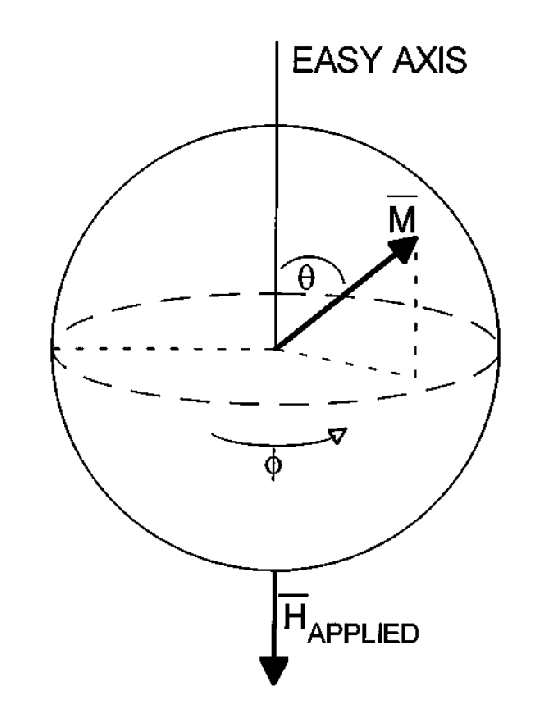
\includegraphics[scale=1]{me20b178_1.eps}
				\end{center}
				\caption{The polar coordinate system showing the magnetization vector M and both the uniaxial anisotropy easy axis and the applied field direction.}
				\label{fig:magnetic_precession} 
			\end{figure}

			\begin{figure}[H]
				\begin{center}
					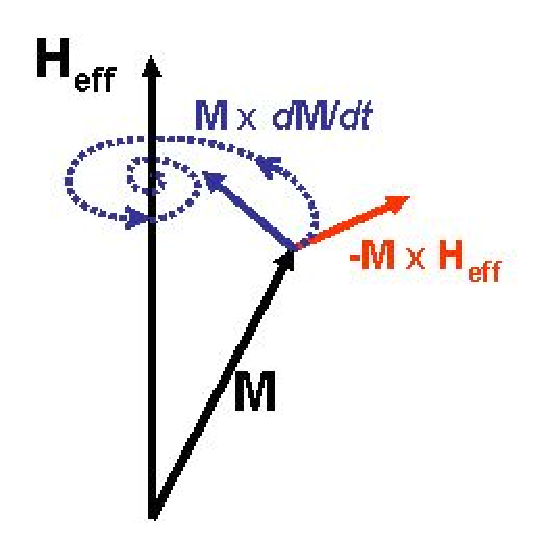
\includegraphics[scale=1]{me20b178_2.eps}
				\end{center}
				\caption{The trajectory of the magnetization \& the terms of the Landau–Lifshitz–Gilbert equation: Precession (red) and damping (blue)}
				\label{fig:damped_magnetic_precession} 
			\end{figure}
		}

		\subsection{Development of the LLG equation}
		{
			\vspace{0.25cm}
			\large
			An earlier, but equivalent, equation (the Landau-Lifshitz equation) was introduced by Landau and Lifshitz in 1935, considering only very small damping:
			\begin{equation}
				\frac{d\overrightarrow{\mathbf{M}}}{dt}=|\gamma| \frac{1}{1+\alpha^{2}}\left(\overrightarrow{\mathbf{M}} \times \overrightarrow{\mathbf{B}}_{\mathrm{eff}}+\frac{\alpha}{M}\left(\overrightarrow{\mathbf{M}} \times\left(\overrightarrow{\mathbf{M}} \times \overrightarrow{\mathbf{B}}_{\mathrm{eff}}\right)\right)\right)
				\label{eqn:LL}
			\end{equation}
			In 1955, Gilbert modified the equation to get eqn.~\ref{eqn:LLG}.
			\newline
			\newline
			An additional term was later added to eqn.~\ref{eqn:LLG} to account for the spin-transfer torque, i.e. the torque induced upon the magnetization by spin-polarized current flowing through the ferromagnet.
		}
	}
